% Created 2026-11-24 Tue 17:42
% Intended LaTeX compiler: pdflatex
\documentclass[letterpaper]{article}

\usepackage[utf8]{inputenc}
\usepackage[T1]{fontenc}
\usepackage{graphicx}
\usepackage{longtable}
\usepackage{wrapfig}
\usepackage{rotating}
\usepackage[normalem]{ulem}
\usepackage{amsmath}
\usepackage{amssymb}
\usepackage{capt-of}
\usepackage{hyperref}
\input{~/Documents/Clases/sample.tex}
\renewcommand{\certificado}{CiberSeguridad}
\renewcommand{\matricula}{AL07083340}
\renewcommand{\docente}{Francisco Gómez Rubio}
\author{Jahil Majorek Casas Sánchez}
\date{24 11 2026}
\title{Informe técnico · Proyecto final de Ciberseguridad}
\hypersetup{
 pdfauthor={Jahil Majorek Casas Sánchez},
 pdftitle={Informe técnico · Proyecto final de Ciberseguridad},
 pdfkeywords={},
 pdfsubject={},
 pdfcreator={},
 pdflang={Spanish}}
\begin{document}

\maketitle
\tableofcontents

Repositorio de trabajo: \href{README.org}{Proyecto-Final/} · \textbf{pendiente de publicar en GitHub} (este entorno no tiene credenciales de publicación).

\begin{abstract}
Este informe continúa el avance del proyecto de ciberseguridad del despacho ficticio
\textbf{Ramírez \& Asociados, S.C.} Tras diagnosticar riesgos, aplicar controles de accesos,
cifrado, respaldos y firewall en la etapa anterior, se evalúa ahora la superficie web
de la organización. Se construyó una aplicación Flask de laboratorio con dos modos:
uno deliberadamente vulnerable y otro corregido. Se reprodujeron y mitigaron
inyección SQL, XSS y control de acceso roto (IDOR/BOLA), y se implementó un mecanismo
de monitoreo y detección como mejora específica (Opción B).

Las pruebas muestran que el payload \texttt{Delta' OR '1'='1' -{}-{}} pasó de devolver 5
expedientes a 0; el script \texttt{<script>alert('XSS-PROYECTO-FINAL')</script>} pasó de
ejecutarse a mostrarse escapado con CSP; y el usuario \texttt{a\_auxiliar} pasó de leer el
expediente de \texttt{s\_tio} (200) a recibir 403. El registro de eventos correlacionó fallos
de login, patrones de ataque y accesos denegados en alertas verificables. Se cierra
con un procedimiento de respuesta a incidentes alineado con el escenario de
ransomware y con la distinción entre acciones probadas y recomendaciones.
\end{abstract}
\section{Resumen ejecutivo}
\label{sec:orgfcd0ee2}

\subsection{Objetivo}
\label{sec:orgb3eee80}

Evaluar vulnerabilidades comunes de aplicaciones web, implementar y validar medidas
de protección, y desarrollar una mejora técnica que fortalezca la seguridad de la
organización seleccionada en el avance.
\subsection{Resultados verificables}
\label{sec:org4bc9848}

\begin{center}
\begin{tabularx}{\textwidth}{X|X|X|X}
Área & Resultado antes & Resultado después & Evidencia\\
\hline
Preparación del entorno & Aplicación y endpoints en 127.0.0.1 & 5 rutas verificadas en cada modo & \href{evidencias/texto/01\_entorno\_endpoints.txt}{01\textsubscript{entorno}\textsubscript{endpoints.txt}}\\
SQL Injection & 5 filas con payload & 0 filas; consulta parametrizada & \href{evidencias/texto/02\_sqli\_validacion.txt}{02\textsubscript{sqli}\textsubscript{validacion.txt}}\\
XSS & Script sin escapar en HTML & \texttt{<script>} escapado + CSP & \href{evidencias/texto/03\_xss\_validacion.txt}{03\textsubscript{xss}\textsubscript{validacion.txt}}\\
IDOR/BOLA & Expediente ajeno 200 & 403 para \texttt{a\_auxiliar}; 200 para propietario & \href{evidencias/texto/04\_idor\_validacion.txt}{04\textsubscript{idor}\textsubscript{validacion.txt}}\\
Registros y detección & Sin correlación & 4 alertas de reglas + panel & \href{evidencias/texto/05\_registros\_monitoreo.txt}{05\textsubscript{registros}\textsubscript{monitoreo.txt}}\\
Mejora organizacional (Opción B) & Sin visibilidad central & Eventos JSON + reglas + panel \texttt{/alertas} & \href{lab/monitoreo/reglas.json}{reglas.json}\\
OWASP ZAP (antes/después) & 3 alto, 20 medio, 19 bajo, 99 informativo & 0 alto, 3 medio, 18 bajo, 111 informativo & \href{evidencias/texto/06\_zap\_antes\_despues.txt}{06\textsubscript{zap}\textsubscript{antes}\textsubscript{despues.txt}}\\
\end{tabularx}
\end{center}
\subsection{Alcance y límites}
\label{sec:org8ec994b}

\begin{itemize}
\item Todo el tráfico se generó contra \texttt{127.0.0.1} (puertos 5000 y 5001). No se escanearon
sistemas de terceros.
\item Los datos, clientes, montos y cuentas son ficticios. Las credenciales se inyectan
por variable de entorno y no se versionan.
\item La versión vulnerable se conserva únicamente como laboratorio; la versión corregida
es la que debe tomarse como referencia de diseño.
\end{itemize}
\section{Contexto de la organización (Actividad 6)}
\label{sec:orgcd9a99e}

\subsection{Ficha institucional}
\label{sec:orgbca7f4a}

\begin{center}
\begin{tabular}{ll}
Campo & Valor\\
\hline
Organización & Ramírez \& Asociados, S.C. (ficticia)\\
Industria & Contabilidad, nómina y asesoría legal para pyMEs\\
Tamaño & 28 empleados, 3 socios, alrededor de 180 clientes\\
Ubicación & Ciudad de México (LFPDPPP; GDPR para clientes internacionales)\\
Servicios críticos & Declaraciones fiscales, nóminas, expedientes contables y legales\\
Datos sensibles & RFC/CURP, ingresos, datos bancarios, nóminas, casos legales\\
\end{tabular}
\end{center}
\subsection{Escenario de ransomware retomado}
\label{sec:org116334f}

Un auxiliar abrió el correo ficticio \texttt{"Factura pendiente de pago.zip"} un viernes a
las 17:40. El archivo cifró el servidor de archivos y, como el NAS de respaldo estaba
montado con las mismas credenciales, también cifró los respaldos. El lunes no se
podían abrir expedientes ni emitir declaraciones: tres días de paro, riesgo de multa
fiscal y una nota de rescate por 2 BTC.
\subsection{Riesgos principales del avance}
\label{sec:org08c2d78}

\begin{center}
\begin{tabular}{llrll}
Riesgo & Activo & P × I & Nivel & Control propuesto en el avance\\
\hline
Permisos amplios en archivos compartidos & Expedientes contables & 20 & Crítico & Mínimo privilegio por grupo\\
NAS con credenciales iguales y montado & Respaldos & 15 & Crítico & Segmentación y "air-gap"\\
Cuentas sin separación de privilegios & Cuentas locales & 9 & Alto & Grupos socio/contador/auxiliar\\
SSH sin MFA & Acceso remoto & 16 & Crítico & TOTP vía \texttt{pam\_google\_authenticator}\\
Correo sin filtrado & Bandeja de entrada & 25 & Crítico & Filtrado, ClamAV y capacitación\\
\end{tabular}
\end{center}
\subsection{Controles previamente implementados y verificados}
\label{sec:orgd2c64b2}

\begin{itemize}
\item MFA TOTP en SSH: \texttt{s\_tio} permitido con contraseña + código; \texttt{c\_contador} y
\texttt{a\_auxiliar} denegados por política PAM.
\item Perfiles funcionales: \texttt{grupo\_socio} (2001), \texttt{grupo\_contador} (2002) y
\texttt{grupo\_auxiliar} (2003), con ACL y SETGID sobre \texttt{/srv/files}.
\item Firewall \texttt{nftables} con política \texttt{drop}, SSH limitado a 3 intentos/minuto y
SMB/CUPS solo desde la red interna.
\item Cifrado LUKS1 en contenedor de prueba y LUKS2 en disco de respaldo.
\item Respaldos diarios con \texttt{rsync}, retención de 90 días y restauración verificada
con \texttt{sha256sum} idéntico.
\item Simulación GoPhish: 5 correos, 5 aperturas, 5 clics y 3 formularios enviados;
tráfico POST capturado con Wireshark.
\end{itemize}
\subsection{Medidas que quedaron como propuestas}
\label{sec:org434c9fa}

\begin{itemize}
\item HTTPS y filtrado de correo para la landing page y la mensajería.
\item Extender MFA a aplicaciones web (no solo SSH). Era una limitación explícita del
avance y motivó la mejora de esta etapa.
\item Diagramas de red propuestos con tres segmentos y NAS aislado.
\item Rotación completa de 90 días (configurada, pero no esperada en el laboratorio).
\end{itemize}

La evidencia de esta etapa previa se resume en
\href{../INFORME\_EVIDENCIAS.md}{INFORME\textsubscript{EVIDENCIAS.md}} y en la carpeta \texttt{../evidencias/}.
\section{Parte A. Evaluación y protección de una aplicación web}
\label{sec:orga0d2064}

\subsection{Actividad 1. Preparación del entorno}
\label{sec:orge4675ef}

Se creó una aplicación Flask única conmutada por la variable \texttt{LAB\_MODE}:

\begin{itemize}
\item \texttt{vulnerable} en \texttt{http://127.0.0.1:5000}: conserva las tres debilidades.
\item \texttt{secure} en \texttt{http://127.0.0.1:5001}: incluye las correcciones y el monitoreo.
\end{itemize}

Cada modo usa su propia base SQLite y su directorio de registros, para que las
pruebas "antes" y "después" no se contaminen mutuamente. Los endpoints verificados
fueron \texttt{/}, \texttt{/health}, \texttt{/login}, \texttt{/buscar}, \texttt{/comentarios}, \texttt{/expediente/<id>},
\texttt{/api/expediente/<id>}, \texttt{/alertas} y \texttt{/api/alertas}.

\begin{figure}[htbp]
\centering
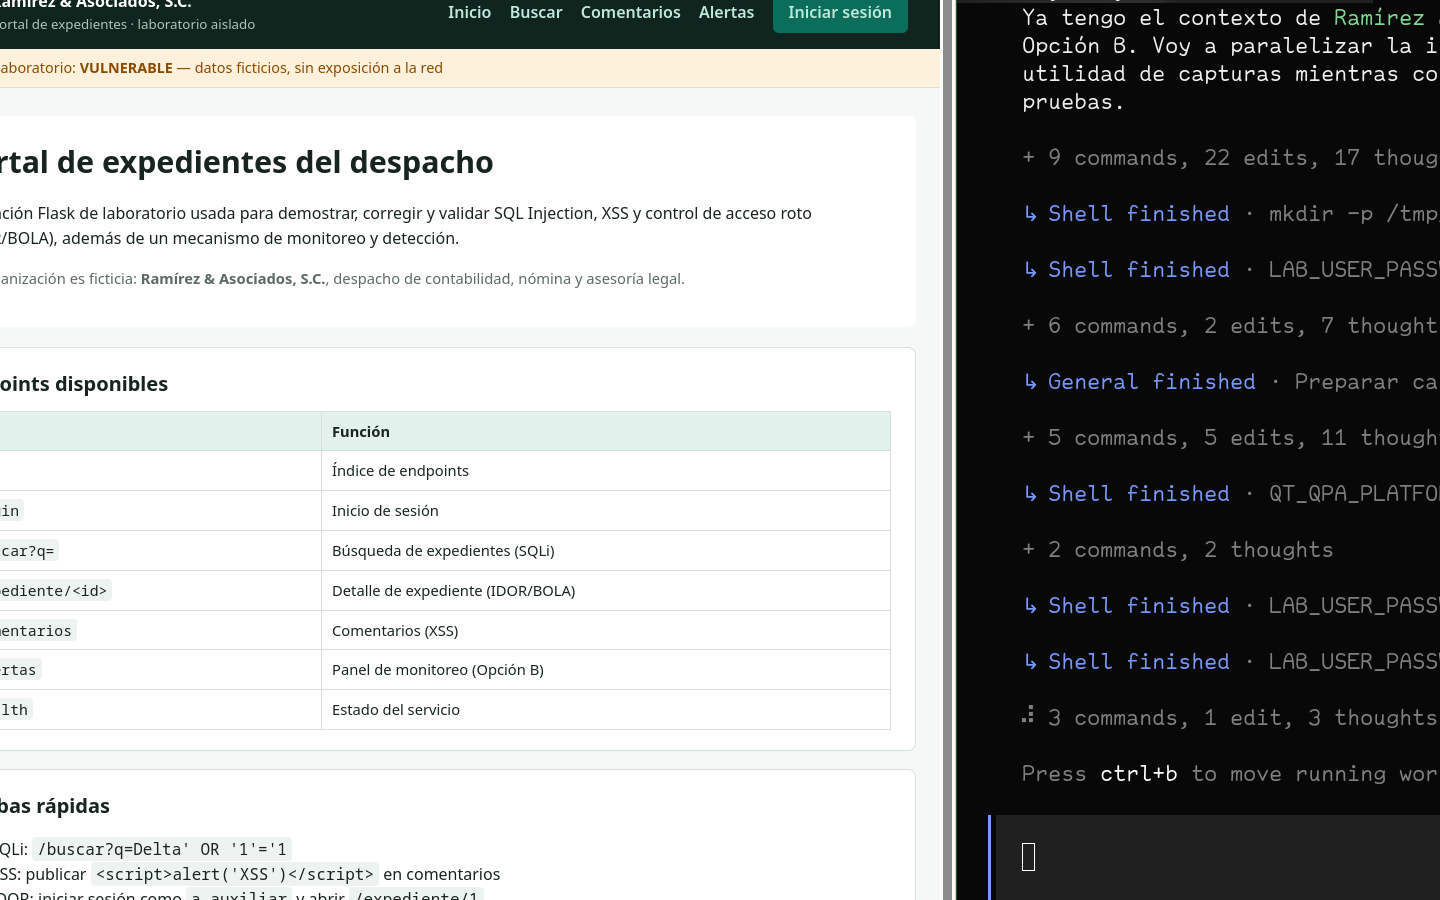
\includegraphics[width=.9\linewidth]{capturas/documento/01_endpoints.png}
\caption{Aplicación de laboratorio en modo vulnerable con el índice de endpoints}
\end{figure}

OWASP ZAP se configuró en modo daemon contra la instancia vulnerable. El procedimiento,
la versión y los informes quedan en \href{lab/zap/README.org}{lab/zap/README.org} y el resumen
legible en \href{evidencias/zap/zap\_resumen.txt}{zap\textsubscript{resumen.txt}}.
\subsection{Metodología de pruebas}
\label{sec:orgb4723bc}

Para cada vulnerabilidad se documentó: componente afectado, descripción, procedimiento,
resultado observado, riesgo e impacto. Después de la corrección se repitió exactamente
la misma petición y se comparó la respuesta. Las pruebas manuales se automatizaron en
\href{lab/pruebas/probar.py}{probar.py}, que regenera los archivos de \texttt{evidencias/texto/}.

\begin{center}
\begin{tabular}{lll}
Herramienta & Uso & Resultado\\
\hline
\texttt{curl} / \texttt{requests} & Reproducción manual de payloads & Antes/después por vulnerabilidad\\
OWASP ZAP & Spider y escaneo activo sobre la app vulnerable & Informes JSON/HTML y resumen\\
Navegador Qt & Evidencia visual de las respuestas & Capturas con \texttt{grim} y \texttt{slurp}\\
\end{tabular}
\end{center}
\subsection{Actividad 2 y 4. Inyección SQL (CWE-89)}
\label{sec:org778f1ce}

\subsubsection{Componente y problema}
\label{sec:org9b7dcb9}

\texttt{/buscar} construía la sentencia con concatenación de texto:

\begin{verbatim}
# ANTES (modo vulnerable)
sql = ("SELECT id, cliente, descripcion, importe FROM expedientes "
       f"WHERE cliente LIKE '%{q}%'")
filas = conn.execute(sql).fetchall()
\end{verbatim}
\subsubsection{Procedimiento}
\label{sec:org2d35105}

\begin{enumerate}
\item Abrir \texttt{/buscar} sin filtro y contar resultados de referencia.
\item Enviar \texttt{q=Delta' OR '1'='1' -{}-{}}; el \texttt{-{}-{}} comenta el cierre de comilla añadido
por la aplicación.
\item Repetir la misma URL en el modo corregido.
\end{enumerate}
\subsubsection{Resultado observado}
\label{sec:org2be9bcc}

En el modo vulnerable la respuesta pasó de 1 expediente ("Constructora Delta") a
\textbf{5 expedientes}, incluidos los propiedad de otros perfiles. En el modo corregido la
misma entrada devolvió \textbf{0 filas}: el payload se comparó como texto literal.

\begin{figure}[htbp]
\centering
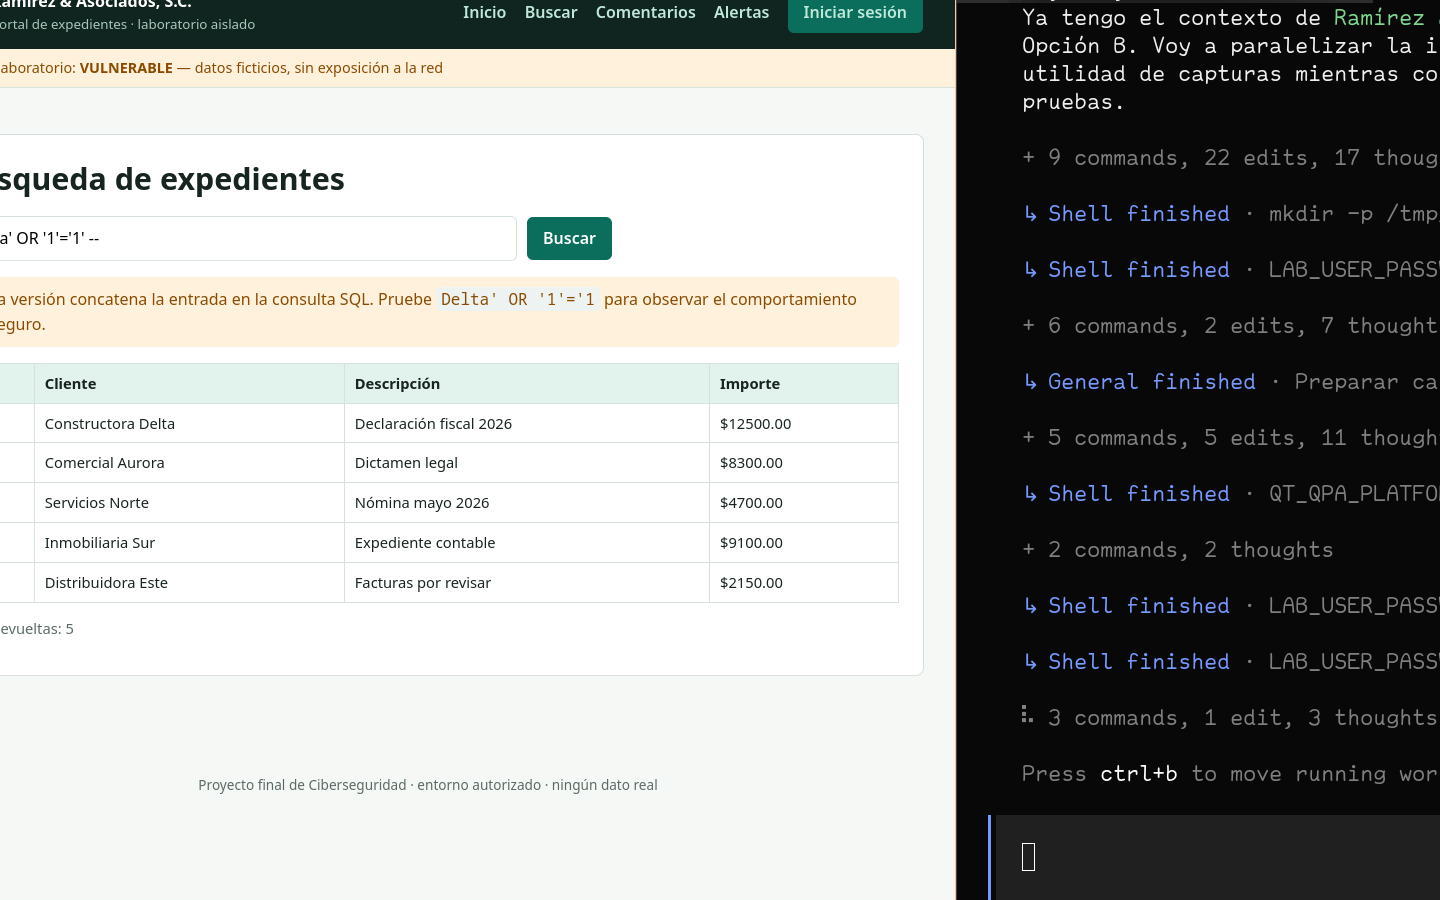
\includegraphics[width=.9\linewidth]{capturas/documento/02_sqli_vulnerable.png}
\caption{SQLi exitosa en la versión vulnerable: se listan los cinco expedientes}
\end{figure}

\begin{figure}[htbp]
\centering
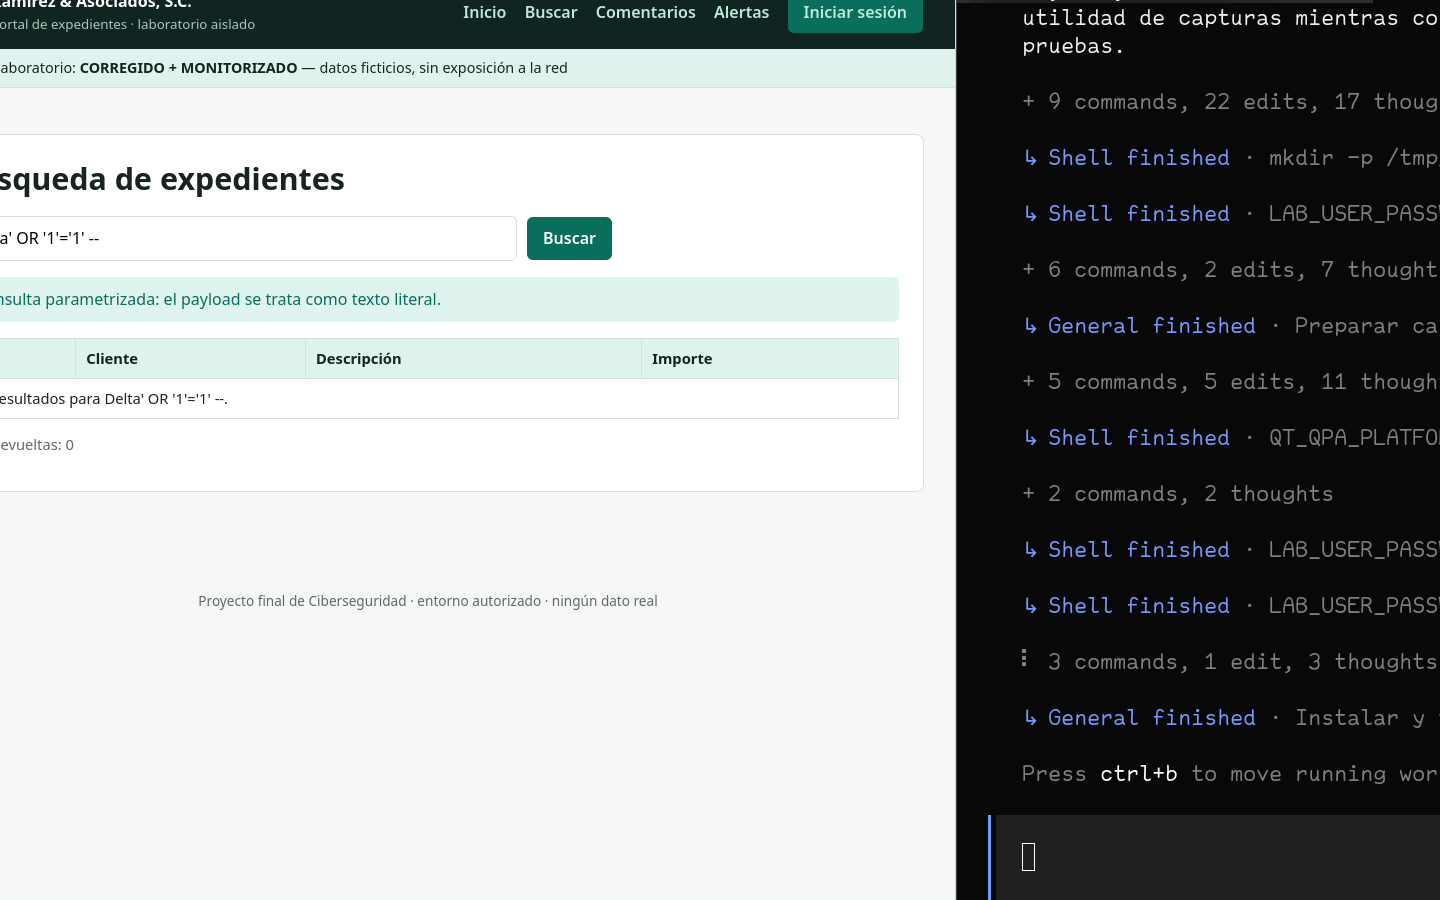
\includegraphics[width=.9\linewidth]{capturas/documento/06_sqli_corregido.png}
\caption{Misma payload en la versión corregida: sin resultados inesperados}
\end{figure}
\subsubsection{Corrección}
\label{sec:org19401af}

\begin{verbatim}
# DESPUÉS (modo seguro): parámetros + validación de longitud
if len(q) > 80:
    abort(400)
filas = conn.execute(
    "SELECT id, cliente, descripcion, importe FROM expedientes "
    "WHERE cliente LIKE ?", (f"%{q}%",)
).fetchall()
\end{verbatim}

Además se registra \texttt{SQLI\_DETECTADO} cuando la entrada coincide con un patrón de
inyección, aunque la consulta parametrizada ya neutralice el efecto.
\subsubsection{Riesgo e impacto y por qué el control reduce el riesgo}
\label{sec:org9b4764d}

Lectura no autorizada de expedientes, posible modificación si el usuario de base de
datos tuviera permisos de escritura y exposición de RFC o montos. La parametrización
separa código de datos: el motor SQLite compila la consulta antes de enlazar el valor,
por lo que las comillas del atacante no pueden alterar la gramática SQL.
\subsection{Actividad 2 y 4. Cross-Site Scripting (CWE-79)}
\label{sec:orgf6df238}

\subsubsection{Componente y problema}
\label{sec:org52d7dd5}

\texttt{/comentarios} almacenaba texto del usuario y la plantilla lo insertaba con \texttt{|safe}:

\begin{verbatim}
<!-- ANTES: Jinja recibe la orden de no escapar -->
{% if modo == 'vulnerable' %}{{ c.texto|safe }}{% else %}{{ c.texto }}{% endif %}
\end{verbatim}
\subsubsection{Procedimiento}
\label{sec:org774ad68}

\begin{enumerate}
\item Iniciar sesión como \texttt{s\_tio} y publicar
\texttt{<script>alert('XSS-PROYECTO-FINAL')</script>}.
\item Recargar \texttt{/comentarios} y buscar la etiqueta sin escapar en el HTML.
\item Repetir en el modo corregido y revisar la cabecera \texttt{Content-Security-Policy}.
\end{enumerate}
\subsubsection{Resultado observado}
\label{sec:orgf84233a}

Antes, el HTML contenía \texttt{<script>} literal y el navegador ejecutaba \texttt{alert()}.
Después, el HTML contiene \texttt{\&lt;script\&gt;} y la cabecera CSP es
\texttt{default-src 'self'; script-src 'self'; object-src 'none'; ...}.

\begin{figure}[htbp]
\centering
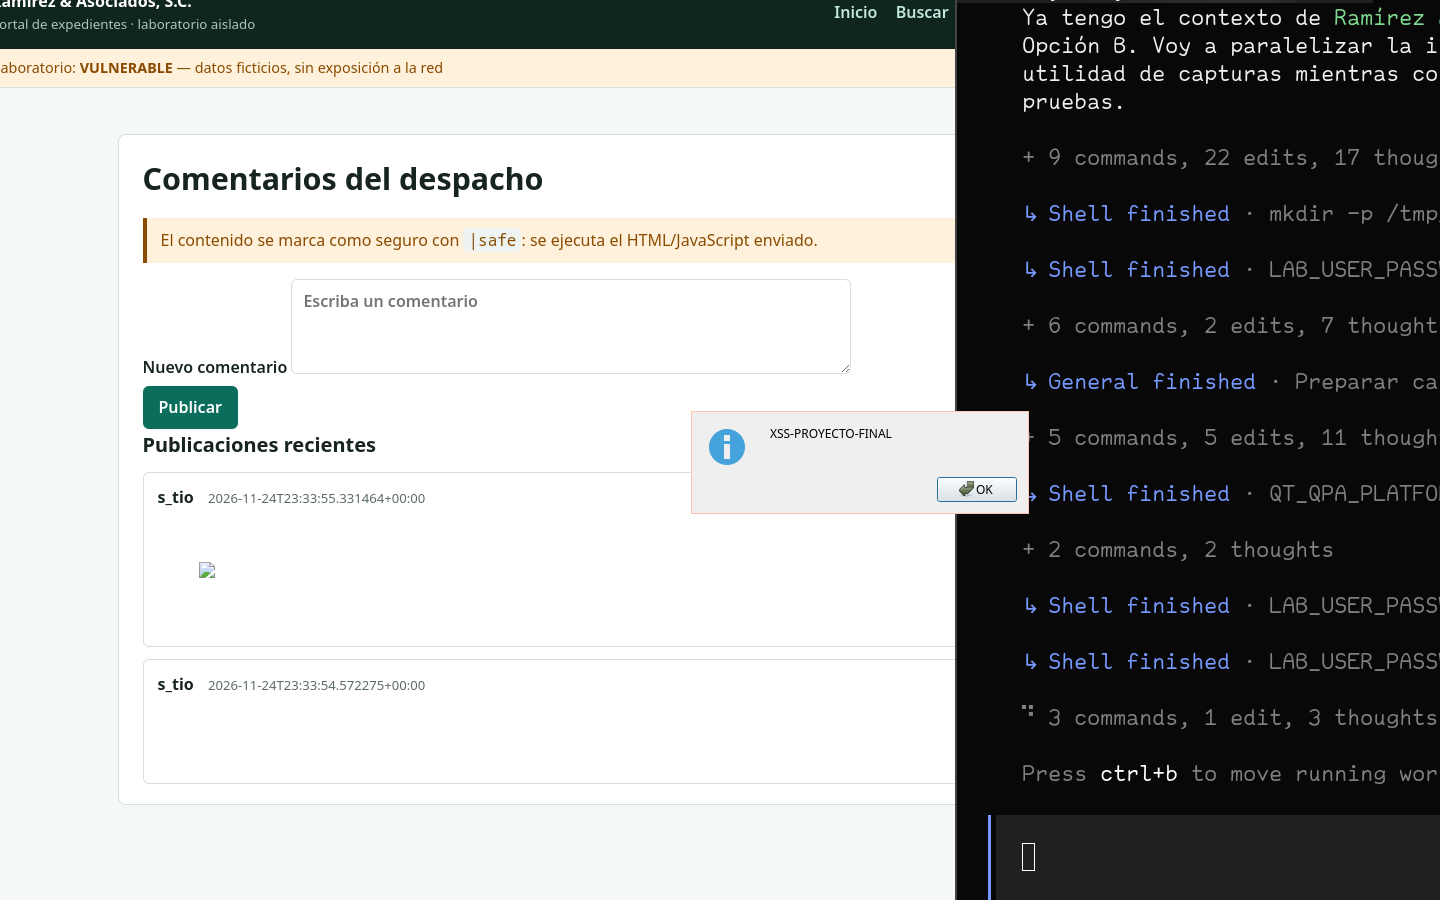
\includegraphics[width=.9\linewidth]{capturas/documento/03_xss_vulnerable.png}
\caption{XSS reflejado en la versión vulnerable}
\end{figure}
\subsubsection{Corrección}
\label{sec:org5ba56d0}

\begin{verbatim}
# La plantilla usa autoescape por defecto en modo seguro: {{ c.texto }}
# Cabecera añadida en after_request:
respuesta.headers["Content-Security-Policy"] = (
    "default-src 'self'; script-src 'self'; object-src 'none'; "
    "base-uri 'none'; frame-ancestors 'none'; form-action 'self'"
)
\end{verbatim}
\subsubsection{Riesgo e impacto y por qué el control reduce el riesgo}
\label{sec:org9b174cc}

Robo de cookie de sesión, acciones suplantadas, phishing dentro del origen legítimo y
desfiguración. El autoescape convierte caracteres especiales en entidades HTML según
el contexto; CSP constituye una segunda capa que bloquearía scripts inline aunque se
filtrara HTML por otra vía.
\subsection{Actividad 2 y 4. Control de acceso roto: IDOR/BOLA (CWE-639)}
\label{sec:org1c8f77b}

\subsubsection{Componente y problema}
\label{sec:org1edee99}

\texttt{/expediente/<id>} y \texttt{/api/expediente/<id>} buscaban el recurso por identificador y lo
entregaban sin comparar \texttt{owner\_id} con el usuario de la sesión.
\subsubsection{Procedimiento}
\label{sec:org5cd2951}

\begin{enumerate}
\item Iniciar sesión como \texttt{a\_auxiliar}.
\item Solicitar \texttt{/expediente/1}, propiedad de \texttt{s\_tio}.
\item Repetir en el modo corregido; verificar además el expediente propio (id 5) y el
acceso de \texttt{s\_tio} al id 1.
\end{enumerate}
\subsubsection{Resultado observado}
\label{sec:org8b938c6}

\begin{center}
\begin{tabular}{llr}
Petición & Vulnerable & Corregido\\
\hline
\texttt{a\_auxiliar} → \texttt{/expediente/1} & 200, datos ajenos & 403\\
\texttt{a\_auxiliar} → \texttt{/api/expediente/1} & 200, JSON ajeno & 403\\
\texttt{a\_auxiliar} → \texttt{/expediente/5} (propio) & 200 & 200\\
\texttt{s\_tio} → \texttt{/expediente/1} (socio) & 200 & 200\\
\end{tabular}
\end{center}

\begin{figure}[htbp]
\centering
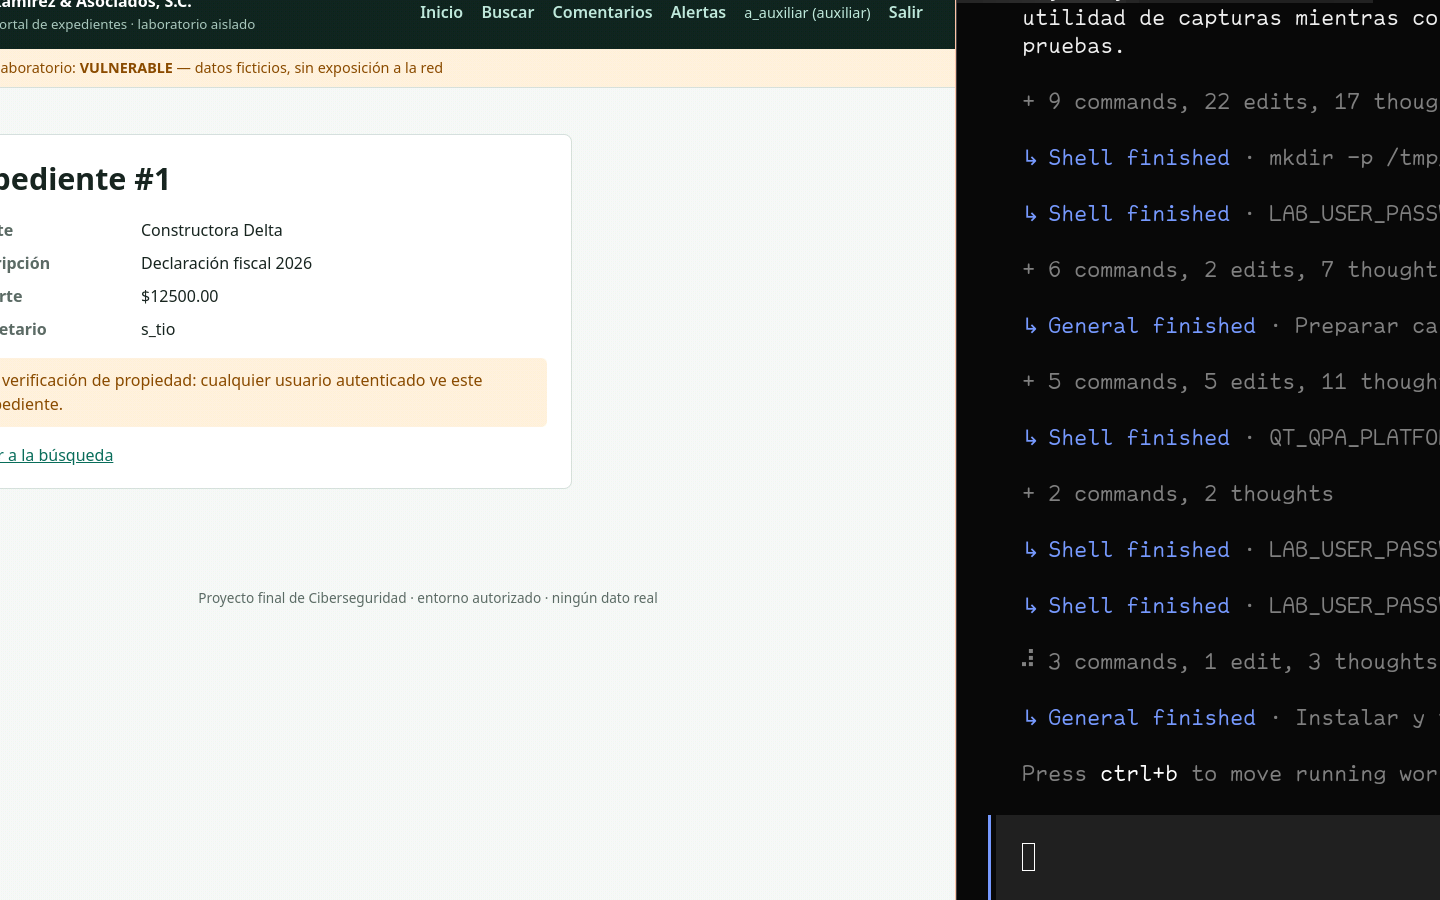
\includegraphics[width=.9\linewidth]{capturas/documento/04_idor_vulnerable.png}
\caption{Acceso indebido a un expediente ajeno en la versión vulnerable}
\end{figure}

\begin{figure}[htbp]
\centering
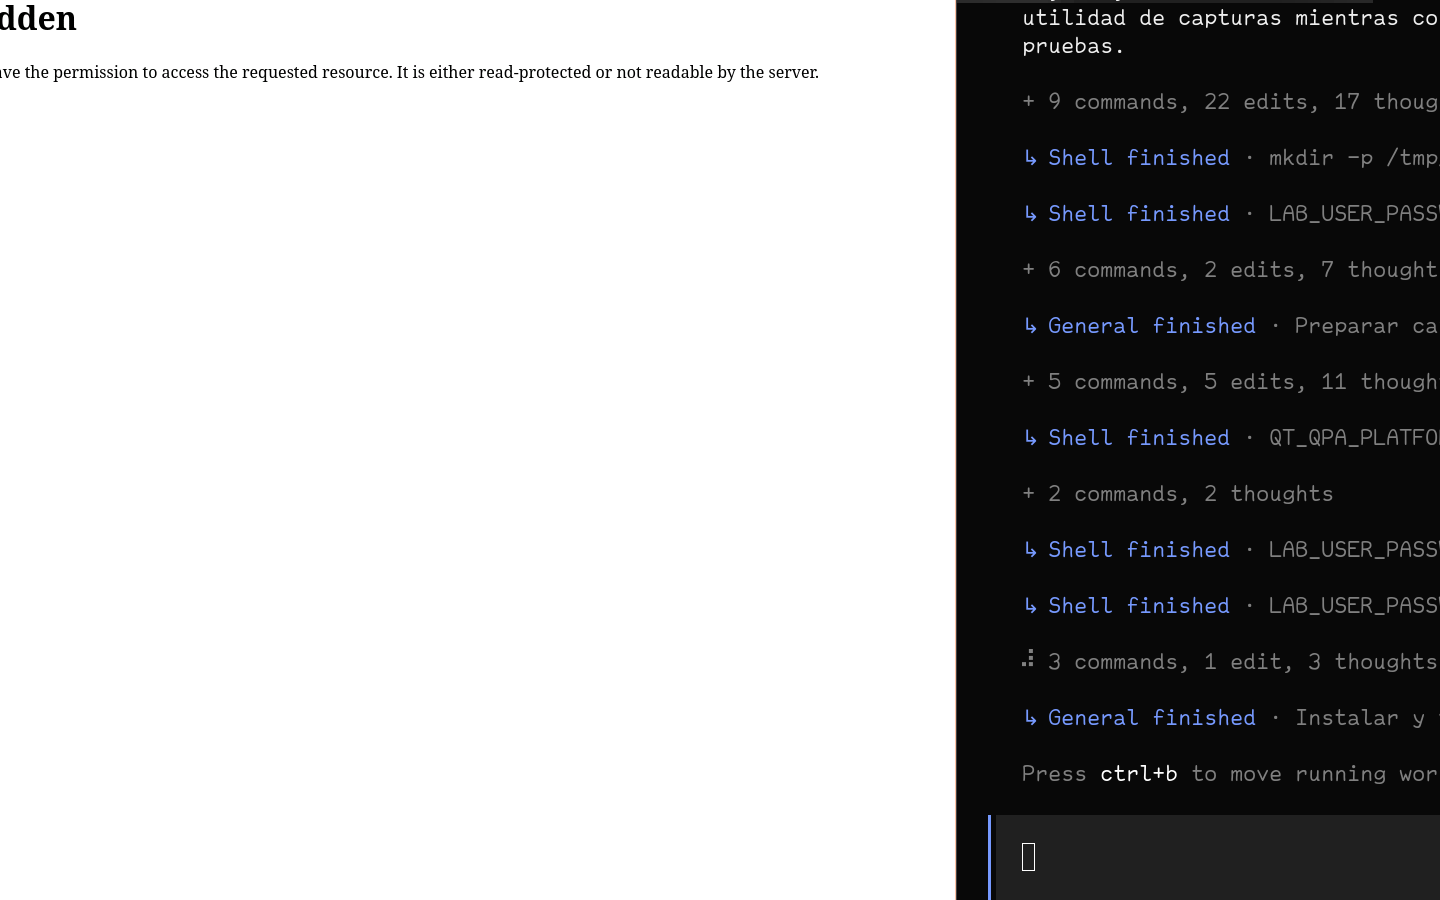
\includegraphics[width=.9\linewidth]{capturas/documento/08_idor_corregido.png}
\caption{Denegación 403 en la versión corregida}
\end{figure}
\subsubsection{Corrección}
\label{sec:orgac678b6}

\begin{verbatim}
permitido = bool(
    fila and usuario
    and (fila["owner_id"] == usuario["id"] or usuario["rol"] == "socio")
)
if not permitido:
    registrar_evento("ACCESO_DENEGADO", "alto", "...", estado=403)
    abort(403)
\end{verbatim}
\subsubsection{Riesgo e impacto y por qué el control reduce el riesgo}
\label{sec:orgfd0b7e7}

Escalada horizontal y vertical, lectura y modificación de expedientes de otros
clientes, incumplimiento de LFPDPPP y pérdida de trazabilidad. La autorización se
ejecuta en el servidor para cada objeto y acción, con denegación por defecto; la
interfaz nunca es la única barrera.
\subsection{Actividad 4. Validación consolidada y resultados de OWASP ZAP}
\label{sec:orgeac6cf2}

\begin{center}
\begin{tabularx}{\textwidth}{X|X|X|X|X}
Vulnerabilidad & Prueba repetida & Antes & Después & Veredicto\\
\hline
SQLi & \texttt{GET /buscar?q=...} & 5 filas & 0 filas & Corregido\\
XSS & Publicar \texttt{<script>alert(...)</script>} & Ejecutado & Escapado + CSP & Corregido\\
IDOR & \texttt{a\_auxiliar} lee expediente 1 & 200 & 403 & Corregido\\
\end{tabularx}
\end{center}

OWASP ZAP 2.17.0 se ejecutó contra el modo vulnerable (spider + escaneo activo) y
reportó \textbf{3 alertas de riesgo alto, 20 medias, 19 bajas y 99 informativas}. Entre las
altas confirmó \texttt{Cross Site Scripting (Persistent)} y \texttt{Reflected} en \texttt{/comentarios} y
\texttt{SQL Injection} en \texttt{/buscar} (respuesta 500 ante \texttt{q='}). El control de acceso roto no
aparece de forma automática porque requiere sesión y comparación de propiedad; por eso
se validó manualmente. Los hallazgos se conservan en
\href{evidencias/zap/zap\_resumen.txt}{zap\textsubscript{resumen.txt}}, con el detalle estructurado en
\texttt{evidencias/zap/zap\_report.json} y el informe HTML en \texttt{evidencias/zap/zap\_report.html}.
Estos resultados se usaron como orientación para priorizar las pruebas manuales; la
confirmación definitiva de cada vulnerabilidad proviene de las peticiones reproducidas.

El mismo escaneo se repitió contra el modo corregido. El resultado fue \textbf{0 alertas altas,
3 medias, 18 bajas y 111 informativas}: desaparecieron SQLi, XSS persistente/reflejado,
la ausencia de CSP (11) y el cabecero anti-clickjacking (6). Quedan tres alertas medias
de ausencia de tokens anti-CSRF en \texttt{/login} y \texttt{/comentarios}, documentadas como riesgo
pendiente. La comparación completa está en
\href{evidencias/texto/06\_zap\_antes\_despues.txt}{06\textsubscript{zap}\textsubscript{antes}\textsubscript{despues.txt}} y el informe
corregido en \href{evidencias/zap/secure/zap\_resumen.txt}{zap\textsubscript{resumen.txt} (secure)}.
ZAP no detectó IDOR/BOLA automáticamente en ninguna de las dos pasadas, por lo que ese
control se validó únicamente con las pruebas manuales autenticadas.

\begin{figure}[htbp]
\centering
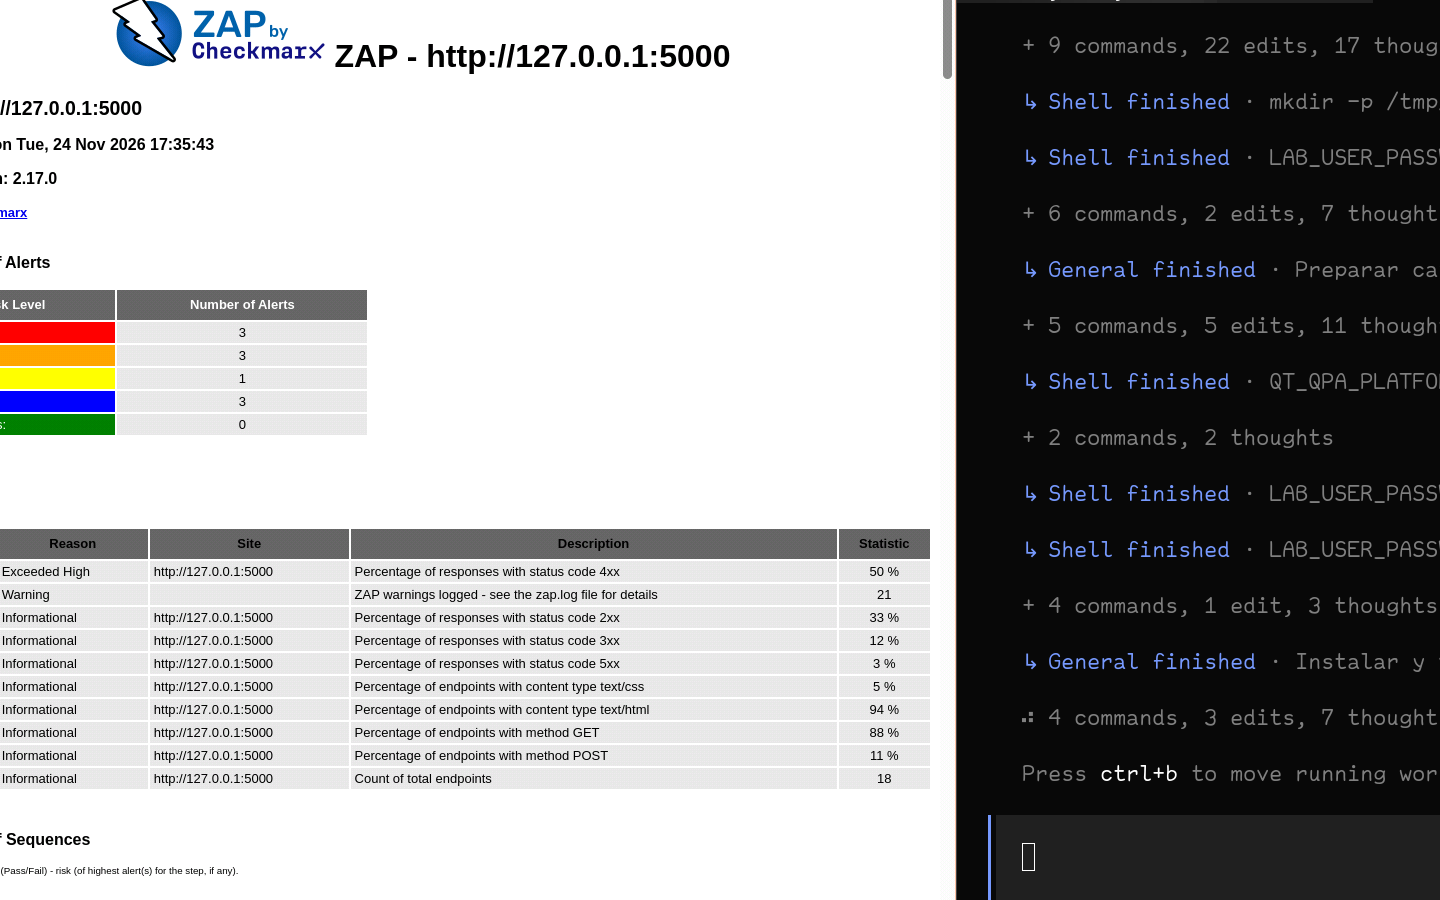
\includegraphics[width=.9\linewidth]{capturas/documento/05_zap_hallazgos.png}
\caption{Resumen de hallazgos de OWASP ZAP sobre la aplicación vulnerable}
\end{figure}
\subsection{Actividad 5. Análisis de registros}
\label{sec:org5966f47}

Se generaron eventos controlados: tres inicios de sesión fallidos, una petición con
patrón SQLi, un comentario con patrón XSS y dos accesos denegados. La aplicación
escribe cada evento en \texttt{logs/security.jsonl} con timestamp UTC, IP, método, ruta,
usuario, resultado y severidad. Las reglas de
\href{lab/monitoreo/reglas.json}{reglas.json} correlacionan esos eventos y escriben
alertas en \texttt{logs/alertas.jsonl}.

La ejecución produjo alertas para los cuatro tipos esperados: fallos de autenticación,
accesos no autorizados, patrón XSS y patrón SQLi. El detalle está en
\href{evidencias/texto/05\_registros\_monitoreo.txt}{05\textsubscript{registros}\textsubscript{monitoreo.txt}}.

Estos registros apoyan la detección porque permiten:

\begin{itemize}
\item Recononstruir la secuencia de una intrusion antes de que exista una alerta de alto nivel.
\item Diferenciar un error de usuario de un patrón repetido de ataque.
\item Medir la eficacia de los controles: el evento de ataque existe aunque la respuesta
sea 403 o la entrada se muestre escapada.
\item Conservar usuario, IP y recurso para la investigación y la notificación.
\end{itemize}
\section{Parte B. Fortalecimiento de la organización}
\label{sec:org41fde2d}

\subsection{Actividad 7. Selección de la mejora}
\label{sec:org8e3d8fc}

Se eligió la \textbf{Opción B: Monitoreo y detección}, porque el avance dejó como limitación
explícita que MFA cubría SSH pero no aplicaciones web, y el escenario de ransomware
mostró que la organización no tenía visibilidad central de eventos de seguridad.
La mejora es verificable: hay eventos persistidos, reglas con umbrales, alertas
correlacionadas y un panel consultable.
\subsection{Actividad 8. Evaluación de resultados}
\label{sec:orgfbe98c4}

\subsubsection{Riesgo que motivó la mejora y situación inicial}
\label{sec:org79bc3a0}

El riesgo es la falta de detección temprana de abuso de credenciales y de accesos
indebidos a expedientes (P × I = 16, Alto en la matriz del avance). Antes de la mejora,
la aplicación devolvía respuestas HTTP correctas pero no dejaba rastro correlacionable:
un atacante podía probar credenciales o iterar identificadores sin generar ninguna
señal para el despacho.
\subsubsection{Solución implementada}
\label{sec:org57d533a}

\begin{center}
\begin{tabular}{lll}
Componente & Archivo & Función\\
\hline
Registro estructurado & \texttt{app/app.py} (\texttt{registrar\_evento}) & JSONL con hora UTC, IP, usuario, ruta, severidad y resultado\\
Reglas de correlación & \href{lab/monitoreo/reglas.json}{reglas.json} & Umbrales por tipo de evento y ventana de 60 s\\
Alertas & \texttt{logs/alertas.jsonl} & Alertas con id, regla, severidad, cantidad y eventos asociados\\
Panel & \texttt{/alertas} y \texttt{/api/alertas} & Consulta restringida al rol socio en el modo seguro\\
Límite de intentos & \texttt{before\_request} en \texttt{/login} & 10 intentos por IP y minuto; evento \texttt{RATE\_LIMIT}\\
\end{tabular}
\end{center}

\begin{figure}[htbp]
\centering
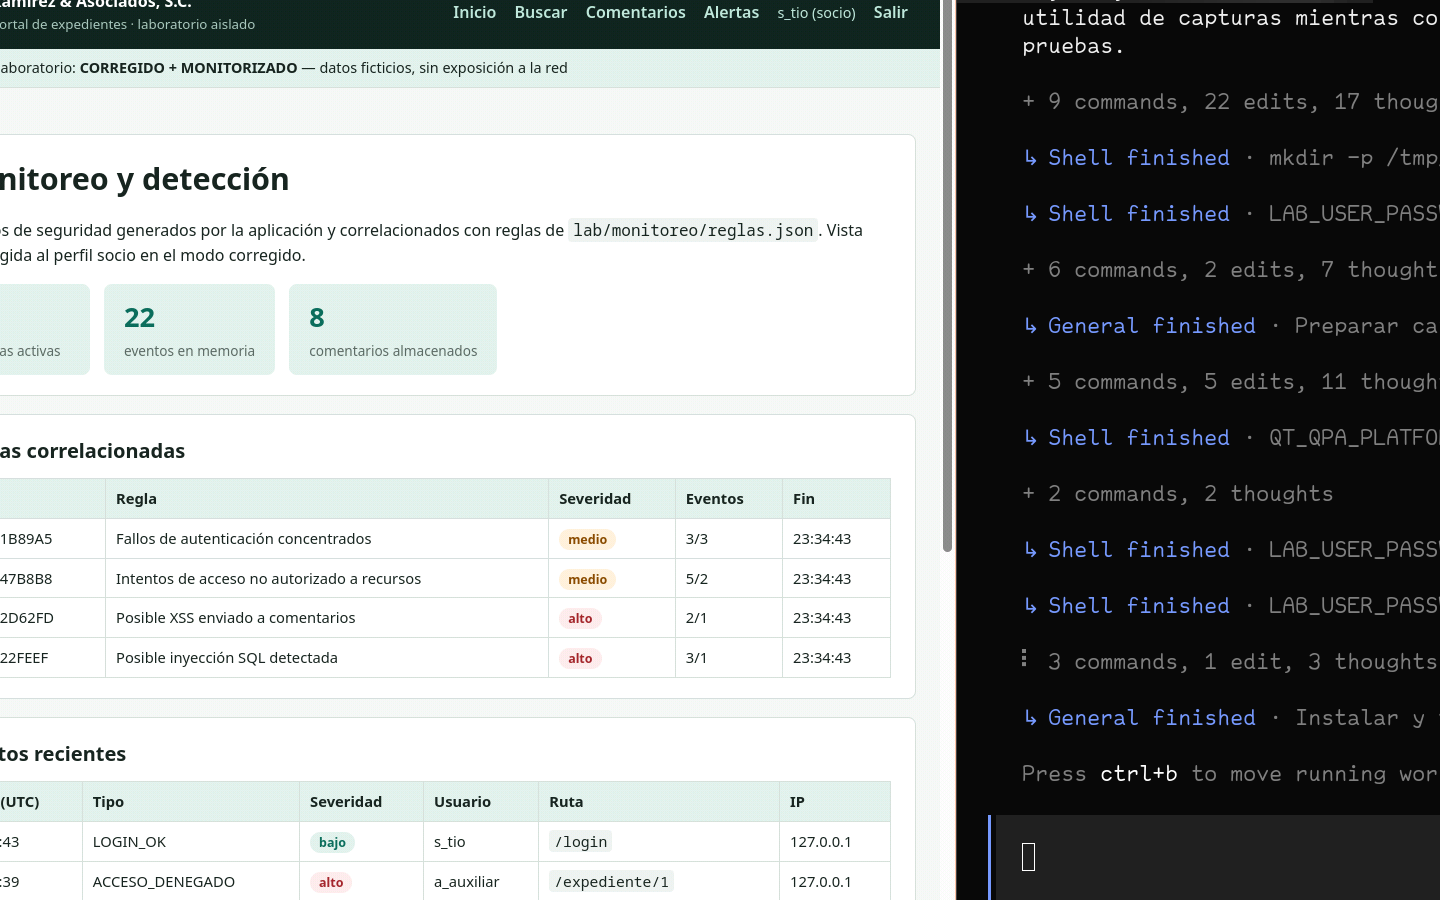
\includegraphics[width=.9\linewidth]{capturas/documento/09_alertas_monitoreo.png}
\caption{Panel de monitoreo y detección con alertas correlacionadas}
\end{figure}
\subsubsection{Pruebas y resultados}
\label{sec:orgf1de57e}

Se repitieron las pruebas de la Parte A sobre el modo corregido y se añadieron eventos
de login fallido, SQLi, XSS y acceso denegado. Resultados:

\begin{itemize}
\item \texttt{LOGIN\_FALLIDO}: 3 eventos → alerta \texttt{LOGIN-001} (severidad media).
\item \texttt{ACCESO\_DENEGADO}: 4 eventos → alerta \texttt{ACCESO-001} (severidad media).
\item \texttt{SQLI\_DETECTADO}: eventos de alto nivel → alerta \texttt{SQLI-001} (severidad alta).
\item \texttt{XSS\_DETECTADO}: eventos de alto nivel → alerta \texttt{XSS-001} (severidad alta).
\item El panel \texttt{/alertas} devolvió 200 para \texttt{s\_tio} y 403 para \texttt{a\_auxiliar}.

Estas cifras corresponden a una ejecución de
\end{itemize}
\href{lab/pruebas/probar.py}{probar.py}; al repetirlo los contadores pueden aumentar,
pero el veredicto de cada regla se mantiene.
\subsubsection{Limitaciones y riesgos pendientes}
\label{sec:org82a9c4c}

\begin{itemize}
\item El registro y el límite de intentos viven en la memoria del proceso: al reiniciar
se pierden las ventanas; el JSONL en disco conserva la historia.
\item No hay envío de alertas a un SIEM ni notificación por correo; el panel requiere
revisión humana.
\item La IP se toma de \texttt{request.remote\_addr}; detrás de un proxy habría que confiar solo
en \texttt{X-Forwarded-For} de proxies conocidos.
\item La detección por patrones puede generar falsos positivos y debe ajustarse con
datos reales antes de aplicar bloqueos automáticos.
\item Quedan pendientes MFA para aplicaciones web, HTTPS y filtrado de correo descritos
en el avance.
\item No se implementaron tokens anti-CSRF: ZAP los reporta en \texttt{/login} y \texttt{/comentarios}.
\item La cabecera \texttt{Server} de Werkzeug divulga la versión; en producción debe ocultarse
mediante un reverse proxy.
\end{itemize}
\section{Actividad 9. Respuesta a incidentes}
\label{sec:org628fb2e}

Procedimiento breve para un incidente de ransomware sobre el despacho, relacionado con
la narrativa de \texttt{"Factura pendiente de pago.zip"}.

\begin{center}
\begin{tabular}{lll}
Etapa & Acciones & Estado\\
\hline
Detección & Alertas por fallos de login, \texttt{SQLI\_DETECTADO}, \texttt{XSS\_DETECTADO} y \texttt{ACCESO\_DENEGADO}; revisión de \texttt{logs/security.jsonl} y del panel \texttt{/alertas}. & \textbf{Probado} en el laboratorio con eventos controlados\\
Análisis & Correlacionar IP, usuario, ruta y timestamp; identificar si hay iteración de \texttt{/expediente/<id>} o patrones SQLi/XSS. & \textbf{Probado} parcialmente: se reconstruyó la secuencia desde los eventos\\
Contención & Negar el acceso al perfil comprometido, bloquear la IP en el firewall y desmontar el volumen de respaldo. & \textbf{Recomendación} probada antes como reglas \texttt{nftables} y política de desmontaje; el bloqueo automático desde este prototipo no se implementó\\
Recuperación & Restaurar expedientes desde el respaldo cifrado verificado con \texttt{sha256sum} y reconstruir la base de la aplicación desde \texttt{init\_db()}. & \textbf{Probado} en el avance para archivos; no se ejecutó un borrado real de la base en esta etapa\\
Verificación & Repetir las tres pruebas de la Parte A, comprobar \texttt{sha256sum} de los archivos restaurados y confirmar que no quedan sesiones activas del usuario comprometido. & \textbf{Probado} para las tres vulnerabilidades; la verificación de sesiones es recomendación\\
\end{tabular}
\end{center}

Secuencia recomendada: ante un pico de \texttt{LOGIN\_FALLIDO} o \texttt{ACCESO\_DENEGADO} se aísla el
servidor de la red, se conservan los registros, se identifica el alcance con las
alertas, se restaura desde el último respaldo íntegro y solo se reintegra el servicio
después de verificar los controles. Las acciones marcadas como recomendación no se
ejecutaron sobre sistemas productivos porque el laboratorio está aislado.
\section{Conclusiones}
\label{sec:org872e895}

\begin{enumerate}
\item Las tres vulnerabilidades exigidas se reprodujeron con peticiones concretas y se
corrigieron en la misma base de código: SQLi con consultas parametrizadas, XSS con
autoescape y CSP, e IDOR con autorización por objeto.
\item La repetición de las mismas pruebas demostró el cambio de comportamiento: 5 → 0
filas, script ejecutado → escapado y 200 → 403 para el usuario sin permiso.
\item OWASP ZAP aportó una vista amplia de hallazgos, pero la validación definitiva fue
manual y reproducible; se priorizó la evidencia demostrable sobre la cantidad de
herramientas.
\item La mejora de monitoreo cerró una brecha del avance: ahora los intentos de ataque
generan eventos y alertas incluso cuando el control defensivo los bloquea.
\item El procedimiento de respuesta distingue con claridad lo probado de lo recomendado,
evitando presentar como implementadas medidas que solo están propuestas.
\item El riesgo residual sigue siendo relevante: el modo vulnerable debe permanecer
aislado, y en producción harían falta HTTPS, MFA en la web, SIEM y revisión
periódica de reglas.
\end{enumerate}
\section{Anexos}
\label{sec:orgc716caf}

\subsection{A. Repositorio y comandos de reproducción}
\label{sec:orgefba509}

El proyecto se entrega como repositorio local en \texttt{\textasciitilde{}/Projects/Ciberseguridad/Proyecto-Final}.
Para publicarlo, crear el repositorio remoto y añadirlo con \texttt{git remote add origin <URL>};
no se publican credenciales ni secretos en este entregable.

\begin{verbatim}
cd ~/Projects/Ciberseguridad/Proyecto-Final
pip install -r app/requirements.txt

LAB_USER_PASSWORD='Laboratorio' lab/run.sh vulnerable 5000 &
LAB_USER_PASSWORD='Laboratorio' lab/run.sh secure 5001 &
LAB_PASSWORD='Laboratorio' python3 lab/pruebas/probar.py

lab/zap/scan.sh http://127.0.0.1:5000 evidencias/zap
lab/zap/scan.sh http://127.0.0.1:5001 evidencias/zap/secure
scripts/exportar.sh
\end{verbatim}
\subsection{B. Índice de evidencias}
\label{sec:org1ab0cf2}

\begin{center}
\begin{tabular}{ll}
Archivo & Contenido\\
\hline
\href{evidencias/texto/01\_entorno\_endpoints.txt}{01\textsubscript{entorno}\textsubscript{endpoints.txt}} & Endpoints y estados HTTP en ambos modos\\
\href{evidencias/texto/02\_sqli\_validacion.txt}{02\textsubscript{sqli}\textsubscript{validacion.txt}} & SQLi antes/después con filas devueltas\\
\href{evidencias/texto/03\_xss\_validacion.txt}{03\textsubscript{xss}\textsubscript{validacion.txt}} & XSS antes/después y cabecera CSP\\
\href{evidencias/texto/04\_idor\_validacion.txt}{04\textsubscript{idor}\textsubscript{validacion.txt}} & Matriz de accesos por usuario y modo\\
\href{evidencias/texto/05\_registros\_monitoreo.txt}{05\textsubscript{registros}\textsubscript{monitoreo.txt}} & Eventos controlados y alertas correlacionadas\\
\href{evidencias/texto/06\_zap\_antes\_despues.txt}{06\textsubscript{zap}\textsubscript{antes}\textsubscript{despues.txt}} & Comparación de hallazgos ZAP antes/después\\
\href{evidencias/zap/zap\_resumen.txt}{zap\textsubscript{resumen.txt}} & Resumen de hallazgos de OWASP ZAP (vulnerable)\\
\href{evidencias/zap/secure/zap\_resumen.txt}{zap\textsubscript{resumen.txt} (secure)} & Resumen de hallazgos de OWASP ZAP (corregido)\\
\href{capturas/documento/}{capturas/documento/} & Capturas usadas en este informe\\
\href{capturas/presentacion/}{capturas/presentacion/} & Capturas preparadas para la presentación ejecutiva\\
\end{tabular}
\end{center}
\subsection{C. Consideraciones éticas}
\label{sec:orgb2e8b9d}

\begin{itemize}
\item Solo se usaron entornos locales autorizados y datos ficticios.
\item No se publican credenciales, secretos ni información personal real.
\item Se permite el uso de IA como apoyo, con revisión y comprensión de las soluciones.
\item La aplicación vulnerable no debe exponerse fuera del laboratorio.
\end{itemize}
\end{document}
